\documentclass{beamer}
\mode<presentation> {
\usepackage{color}
\definecolor{bottomcolour}{rgb}{0.21,0.11,0.21}
\definecolor{middlecolour}{rgb}{0.21,0.11,0.21}
\setbeamercolor{structure}{fg=white}
\setbeamertemplate{frametitle}[default]%[center]
\setbeamercolor{normal text}{bg=black, fg=white}
\setbeamertemplate{background canvas}[vertical shading]
[bottom=bottomcolour, middle=middlecolour, top=black]
\setbeamertemplate{items}[circle]
\setbeamertemplate{navigation symbols}{} %no nav symbols
\setbeamercolor{block title}{use=structure,fg=white,bg=structure.fg!50!red!50!blue!100!green}
\setbeamercolor{block body}{parent=normal text,use=block title,bg=block title.bg!5!white!10!bg,fg=white}
\setbeamertemplate{navigation symbols}{}
}
\usepackage{graphicx} 
\usepackage{booktabs} 
\usepackage[utf8]{inputenc}  
\usepackage[T1]{fontenc}  
\usepackage{geometry}     
%\usepackage[francais]{babel} 
\usepackage{eurosym}
\usepackage{verbatim}
\usepackage{ragged2e}
\justifying

%%%%%%%%%%%%%%%%%%%%%%%%%%%%%%%%%%%%%%%%%%%%%%%%%%%%%%%%%%%%%%%%
%% ccBeamer 0.1, 2007-07-02                                   %%
%% Written by Sebastian Pipping <webmaster@hartwork.org>      %%
%% ---------------------------------------------------------- %%
%% Licensed under Creative Commons Attribution-ShareAlike 3.0 %%
%% http://creativecommons.org/licenses/by-sa/3.0/             %%
%%%%%%%%%%%%%%%%%%%%%%%%%%%%%%%%%%%%%%%%%%%%%%%%%%%%%%%%%%%%%%%%


%% Images
\newcommand{\CcImageBy}[1]{%
	
\includegraphics[scale=#1]{creative_commons/cc_by_30.pdf}%
}
\newcommand{\CcImageCc}[1]{%
	
\includegraphics[scale=#1]{creative_commons/cc_cc_30.pdf}%
}
\newcommand{\CcImageDevNations}[1]{%
	
\includegraphics[scale=#1]{creative_commons/cc_dev_nations_30.pdf}%
}
\newcommand{\CcImageNc}[1]{%
	
\includegraphics[scale=#1]{creative_commons/cc_nc_30.pdf}%
}
\newcommand{\CcImageNd}[1]{%
	
\includegraphics[scale=#1]{creative_commons/cc_nd_30.pdf}%
}
\newcommand{\CcImagePd}[1]{%
	
\includegraphics[scale=#1]{creative_commons/cc_pd_30.pdf}%
}
\newcommand{\CcImageSa}[1]{%
	
\includegraphics[scale=#1]{creative_commons/cc_sa_30.pdf}%
}
\newcommand{\CcImageSampling}[1]{%
	
\includegraphics[scale=#1]{creative_commons/cc_sampling_30.pdf}%
}
\newcommand{\CcImageSamplingPlus}[1]{%
	
\includegraphics[scale=#1]{creative_commons/cc_sampling_plus_30.pdf}%
}


%% Groups
\newcommand{\CcGroupBy}[1]{% zoom
	\CcImageBy{#1}%
}
\newcommand{\CcGroupByNc}[2]{% zoom, gap
	\CcImageBy{#1}\hspace*{#2}\CcImageNc{#1}%
}
\newcommand{\CcGroupByNcNd}[2]{% zoom, gap
	\CcImageBy{#1}\hspace*{#2}\CcImageNc{#1}\hspace*{#2}\CcImageNd{#1}%
}
\newcommand{\CcGroupByNcSa}[2]{% zoom, gap
	\CcImageBy{#1}\hspace*{#2}\CcImageNc{#1}\hspace*{#2}\CcImageSa{#1}%
}
\newcommand{\CcGroupByNd}[2]{% zoom, gap
	\CcImageBy{#1}\hspace*{#2}\CcImageNd{#1}%
}
\newcommand{\CcGroupBySa}[2]{% zoom, gap
	\CcImageBy{#1}\hspace*{#2}\CcImageSa{#1}%
}
\newcommand{\CcGroupDevNations}[1]{% zoom
	\CcImageDevNations{#1}%
}
\newcommand{\CcGroupNcSampling}[2]{% zoom, gap
	\CcImageNc{#1}\hspace*{#2}\CcImageSampling{#1}%
}
\newcommand{\CcGroupPd}[1]{% zoom
	\CcImagePd{#1}%
}
\newcommand{\CcGroupSampling}[1]{% zoom
	\CcImageSampling{#1}%
}
\newcommand{\CcGroupSamplingPlus}[1]{% zoom
	\CcImageSamplingPlus{#1}%
}


%% Text
\newcommand{\CcLongnameBy}{Attribution}
\newcommand{\CcLongnameByNc}{Attribution-NonCommercial}
\newcommand{\CcLongnameByNcNd}{Attribution-NoDerivs}
\newcommand{\CcLongnameByNcSa}{Attribution-NonCommercial-ShareAlike}
\newcommand{\CcLongnameByNd}{Attribution-NoDerivs}
\newcommand{\CcLongnameBySa}{Attribution-ShareAlike}

\newcommand{\CcNote}[1]{% longname
	This work is licensed under the \textit{Creative Commons #1 3.0 License}.%
}


\title[De l'importance de l'éducation populaire au numérique]{De l'importance de l'éducation populaire au numérique}
\author{JDLL 2016}
\author{Genma}

\begin{document}

%% Titlepage
\begin{frame}
	\titlepage
	\vfill
	\begin{center}
		\CcGroupByNcSa{0.83}{0.95ex}\\[2.5ex]
		{\tiny\CcNote{\CcLongnameByNcSa}}
		\vspace*{-2.5ex}
	\end{center}
\end{frame}



%====================================POURQUOI=========================================
\begin{frame}
\begin{center}
\Huge {Accessibilité}
\end{center}
\end{frame}

%--------------------------------------------------------------------------------
\begin{frame}
\frametitle{Accessibilité}

\begin{block}{Visuelle}
\justifying{
\begin{itemize}
\item Est-ce que tout le monde arrive à lire la présentation?
\item Elle est disponbible en ligne, pas la peine de prendre de notes :-)
\end{itemize}}
\end{block}

\begin{center}

\includegraphics[scale=0.4]{./images/accessibilite_v2.jpg}
\end{center}


\begin{block}{Auditive}
\begin{itemize}
\justifying{
\item Je parle vite. Très vite.
\item Merci de me faire signe pour me demander de ralentir, d'articuler.
}
\end{itemize}
\end
{block}
\end{frame}

\begin{frame}
\begin{center}
\Huge {C'est parti :-)}
\end{center}
\end{frame}

\begin{frame}
\frametitle{
\includegraphics[scale=0.4]{./images/Genma.jpg} \ \ \  A propos de moi  }
\begin{columns}[c] 
\column{.55\textwidth} 
\textbf{Où me trouver sur Internet?}
\begin{itemize}
\item Le Blog de Genma : http://genma.free.fr
\item Twitter @genma
\end{itemize}
\column{.5\textwidth} 
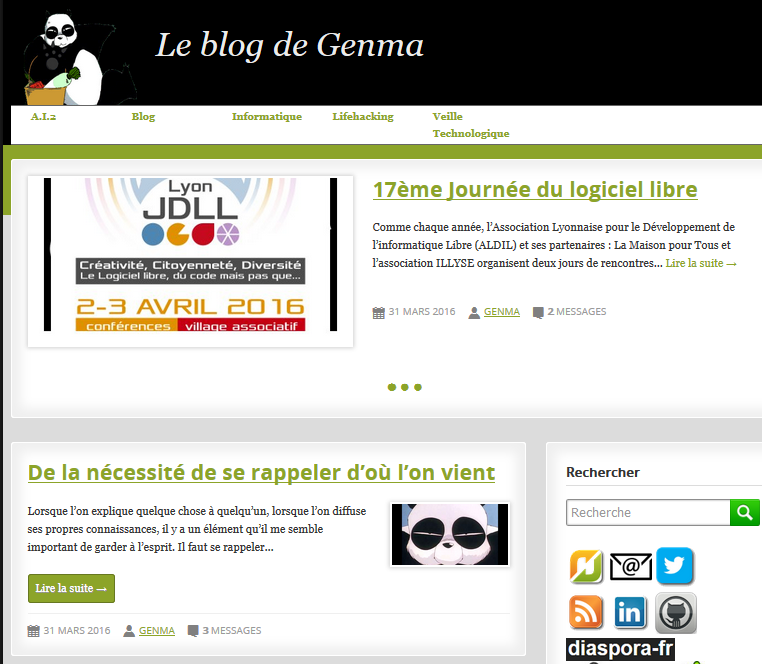
\includegraphics[scale=0.4] {./images/blog.png} 
\end{columns}
\end{frame}

%--------------------------------------------------------------------------------
\begin{frame}
\frametitle{Qui je suis?}

\begin{block}{Une expérience d'\emph{autodidacte}}
\begin{itemize}
\justifying{
\item Je ne suis pas \emph{informaticien} (même si je travaille dans le domaine, je suis Biologiste de formation universitaire).
\item Je suis \emph{libriste} depuis 2003. (Merci Framasoft!)
}
\end{itemize}
\end{block}

\begin{block}{Une expérience de \emph{vulgarisateur}}
\justifying{
\begin{itemize}
\justifying{
\item Formations, conférences et ateliers destinés au grand public, des libristes, des journalistes ou à des geeks hackitvistes...
\item Différents activités dans le milieu associatif libriste (Ubuntu, Framasoft, FirefoxOS, Café vie privée etc.)
}
\end{itemize}
}\end{block}
\end{frame}

%====================================POURQUOI=========================================
\begin{frame}
\begin{center}
\Huge {Pourquoi cette présentation?}
\end{center}
\end{frame}

%--------------------------------------------------------------------------------
\begin{frame}
\frametitle{Pourquoi cette présentation?}

\begin{block}{L’Informatique et Internet sont partout dans nos vies quotidiennes}
\justifying{
Tout à chacun soit à même de s’approprier les connaissances nécessaires et suffisantes pour comprendre ces outils qui changent les fondements mêmes de notre société, dans notre accès à l’information, aux connaissances, au partage, à la communication...}\end{block}

\begin{block}{Importance de la communication et de la vulgarisation}
\justifying{
\begin{itemize}
\item pour que l'éducation populaire se fasse ;
\item que l'on ne pense plus "RTFM" ;
\item que chacun et chacune aura les moyens de s'approprier le numérique et de comprendre les enjeux (neutralité du net, importance de la vie privée, lutte contre les GAFAM etc.)
\end{itemize}
}\end{block}
\end{frame}

%==================================COMMENT==================================================
\begin{frame}
\begin{center}
\Huge {Comment éduquer au numérique?}
\end{center}
\end{frame}

%--------------------------------------------------------------------------------
\begin{frame}
\frametitle{Définir le numérique}

\begin{block}{Un nouveau savoir fondamental, au même titre que parler, lire, écrire et compter}
\justifying{
Mais que veut dire le numérique ? Être au courant des dernières tendance et savoir s'adapter ? Coder ? Gérer un réseau ? Maîtriser les fichiers Multimédia ?
}\end{block}
\end{frame}
 
%--------------------------------------------------------------------------------
\begin{frame}
\frametitle{}
\begin{block}{Ce qu'il faut faire...}
\justifying{
\begin{itemize}
\item Servir de facilitateur 
\item Faire de l'éducation populaire
\item Partager ses connaissances...
\end{itemize}
}\end{block}

\begin{block}{Dans quel but?}
\justifying{
\begin{itemize}
\item Apprendre aux gens à être acteurs du web
\item Créer du contenu en dehors des réseaux sociaux (Facebook) (par exemple)
\end{itemize}
}\end{block}
\justifying{=> D'une façon générale il faut sensibilier.}
\end{frame}

%--------------------------------------------------------------------------------
\begin{frame}
\frametitle{Quelques conseils}

\begin{block}{Se rappeler d'où l'on vient}
\justifying{
On a tous et toutes été des débutants. Et on l'est dans BEAUCOUP d'AUTRES domaines.
}\end{block}

\begin{block}{Respecter l'autre}
\justifying{
\begin{itemize}
\item Comprendre ses besoins, attente, demande et être à l'écoute de ses demandes
\item Il faut se mettre à son niveau
\item Il faut être patient, pédagogue....
\item \emph{Pas de propos sexiste, mysogine, excluant}...
\end{itemize}
}\end{block}
\justifying{=> Et d'une façon générale, arrêter l'intégrisme...}
\end{frame}

%=================================  QUOI  ====================================
\begin{frame}
\begin{center}
\Huge{Il faut sortir de notre tour d'ivoire!}\\ ~\\

\includegraphics[scale=0.4]{./images/L_Histoire_sans_Fin.jpg}
\end{center}
\end{frame}

\begin{frame}
\begin{center}
\Huge {Sous quelles formes?}
\end{center}
\end{frame}

\begin{frame}
\begin{center}
\Huge {Utiliser un vocabulaire adapté}
\end{center}
\end{frame}

%-----------------------------------------------
\begin{frame}
\Huge{On peut dire Linux et même Ubuntu...}
\begin{columns}[c] 
\column{.55\textwidth} 
\begin{center}

\includegraphics[scale=1] {./images/gnu.jpg} 
\end{center}
\column{.5\textwidth} 
\begin{center}

\includegraphics[scale=1] {./images/linux.jpg} 
\end{center}
\end{columns}
\end{frame}


%-----------------------------------------------
\begin{frame}
\begin{center}
\huge{Et ce même si ça déplait à RMS...}

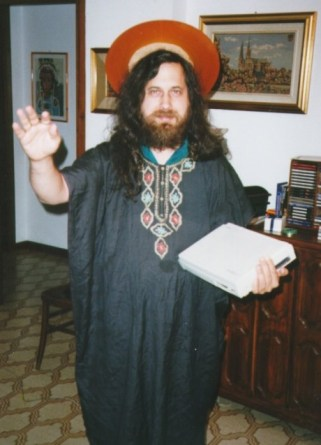
\includegraphics[scale=0.5]{./images/saintignucius.jpg}
\end{center}
\end{frame}

%-----------------------------------------------
\begin{frame}
\begin{center}
\Huge{Parler de coffre-fort numérique}
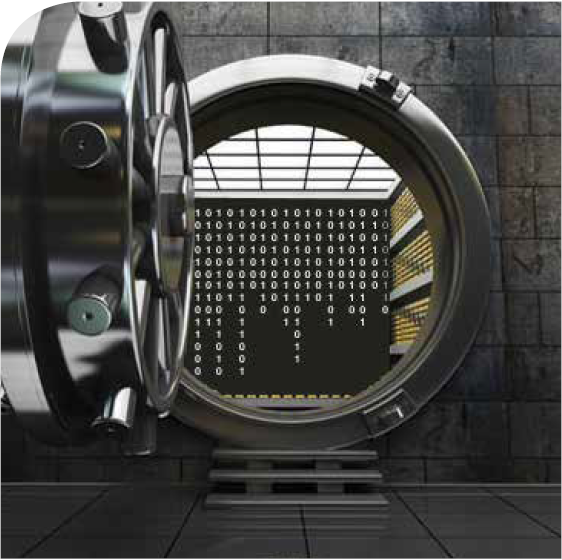
\includegraphics[scale=0.5]{./images/coffre_fort_numerique.png}
\end{center}
\end{frame}

%-----------------------------------------------
\begin{frame}
\begin{center}
\Huge{Acceptez que l'on dise \emph{crypté}}
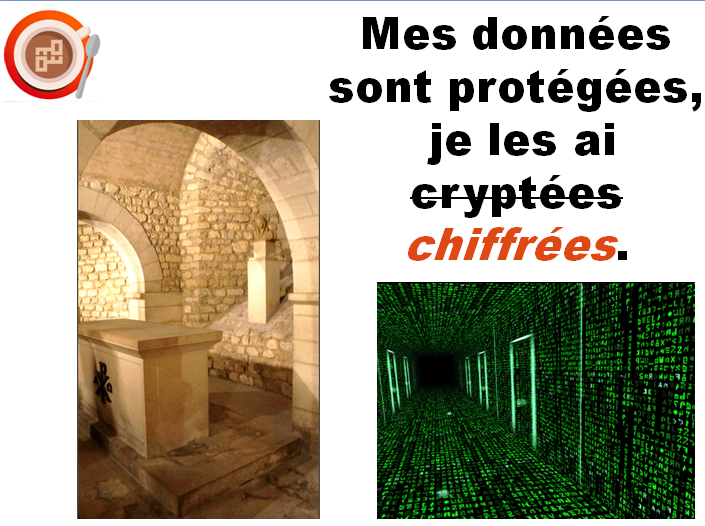
\includegraphics[scale=0.5]{./images/chiffrees_vs_cryptees.png}
\end{center}
\end{frame}

%-----------------------------------------------
\begin{frame}
\begin{center}
\Huge{Utiliser des analogies \\comme celles des recettes de cuisine...}
\end{center}
\end{frame}

%-----------------------------------------------
\begin{frame}
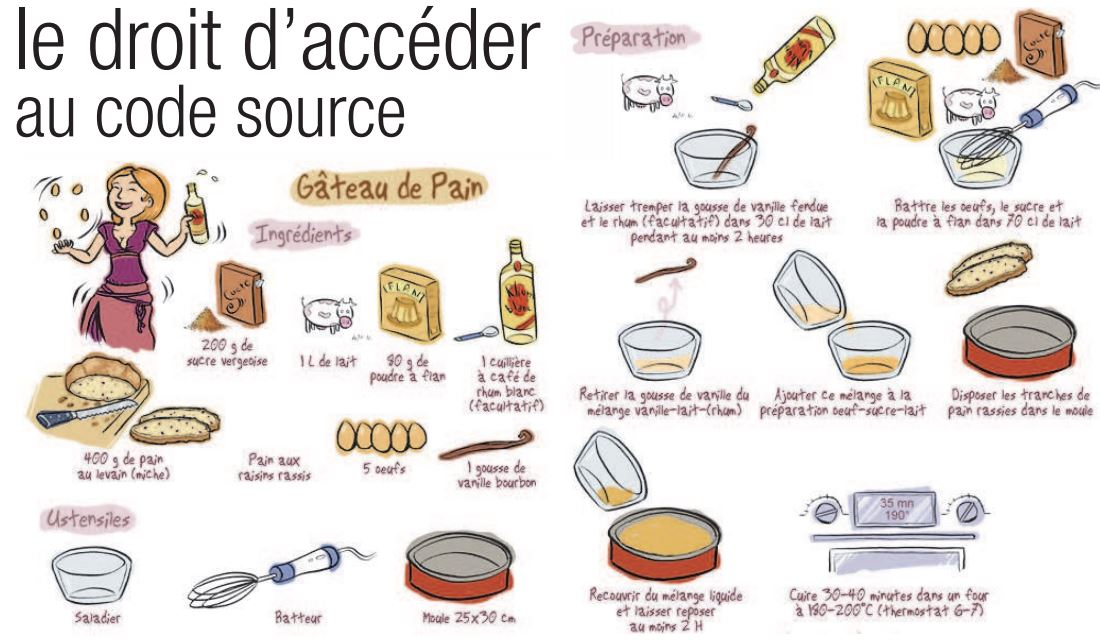
\includegraphics[scale=0.6] {./images/Cuisine01.jpg} 
\end{frame}
\begin{frame}
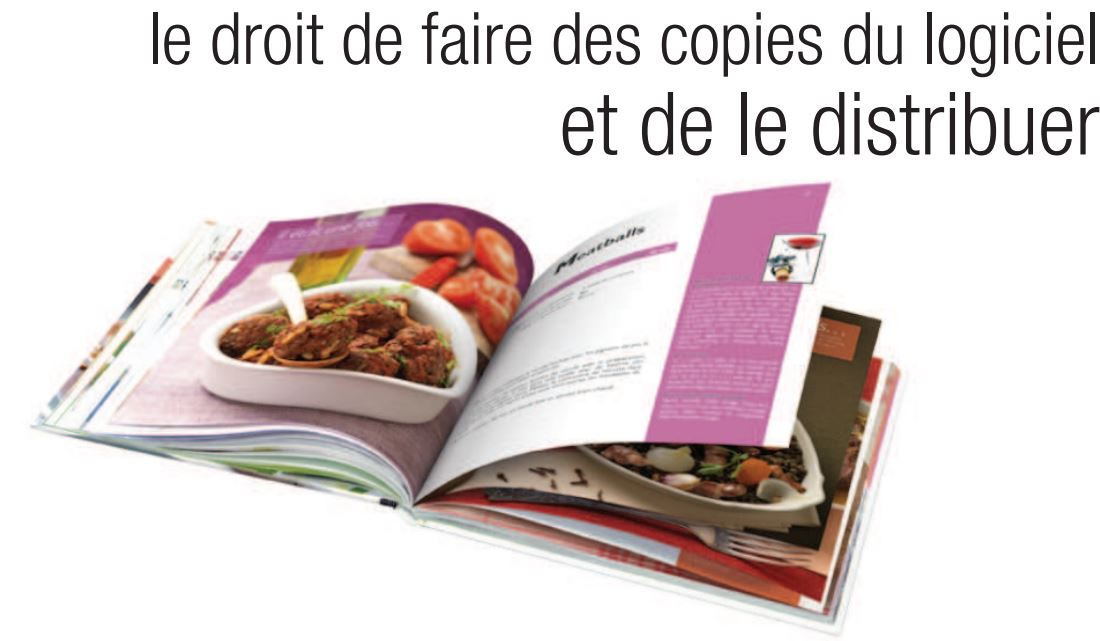
\includegraphics[scale=0.5] {./images/Cuisine02.jpg} 
\end{frame}
\begin{frame}
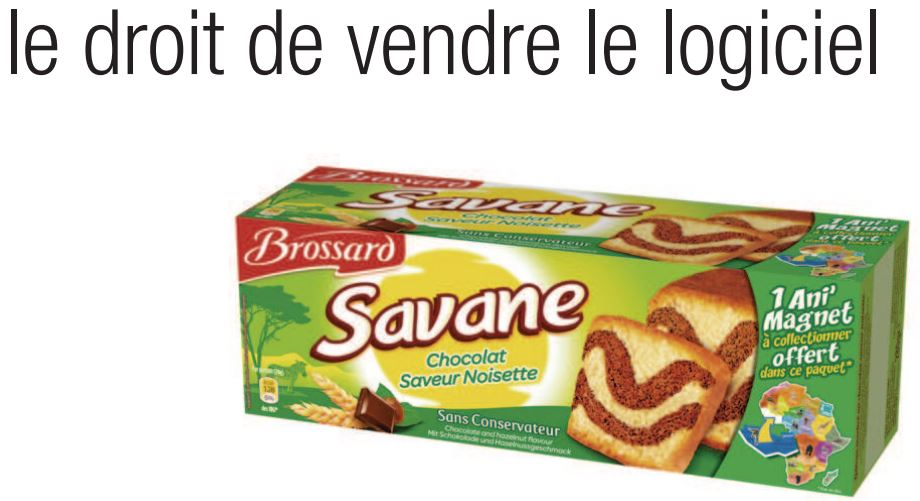
\includegraphics[scale=0.6] {./images/Cuisine03.jpg} 
\end{frame}
\begin{frame}
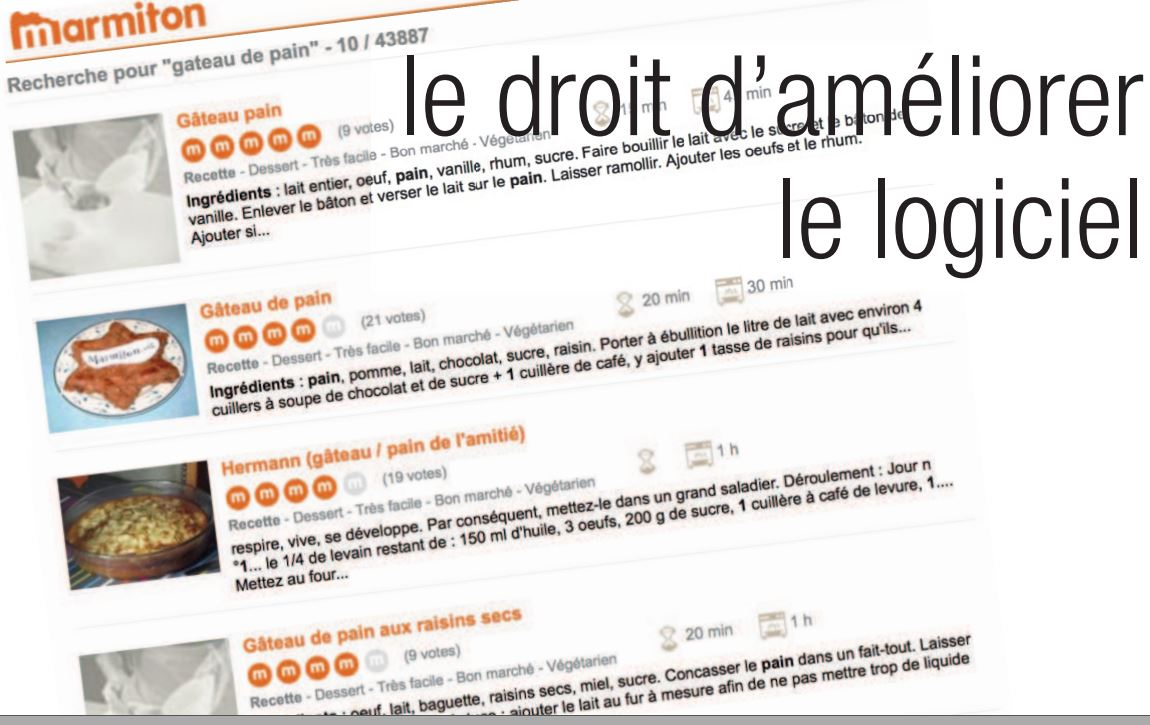
\includegraphics[scale=0.48] {./images/Cuisine04.jpg} 
\end{frame}

%-----------------------------------------------
\begin{frame}
\begin{center}
\Huge{Il faut utiliser une communication accessible}
\end{center}
\end{frame}

%----------------------------------------------------------------------------------------
\begin{frame}
\frametitle{Pour les enfants}
\begin{center}

\includegraphics[scale=0.5] {./images/scractch_4_kids.jpg}

\includegraphics[scale=0.5] {./images/python_4_kids.jpg}
\end{center}
\end{frame}


%----------------------------------------------------------------------------------------
\begin{frame}
\frametitle{Un visuel qui interpelle lié à la culture populaire}
\begin{center}
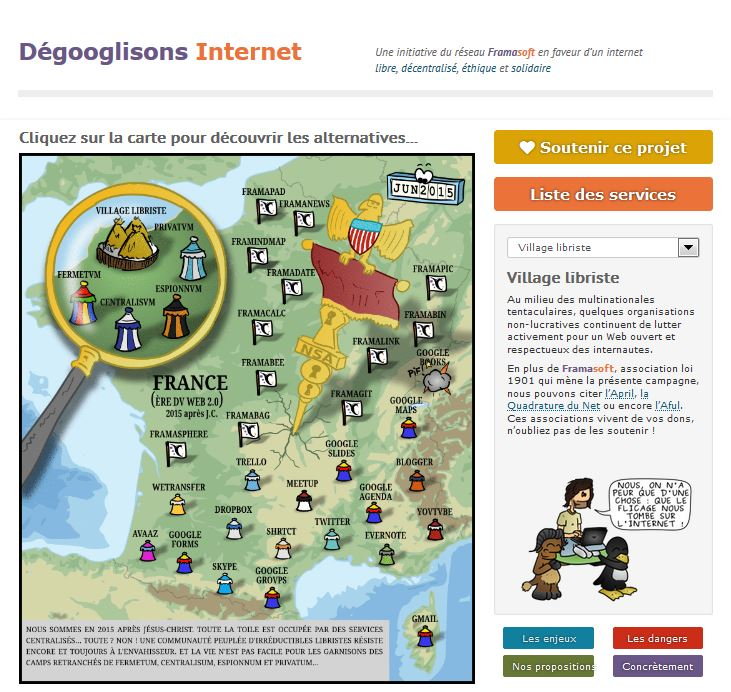
\includegraphics[scale=0.6] {./images/framasoft_degogglisons.jpg}
\end{center}
\end{frame}

%----------------------------------------------------------------------------------------
\begin{frame}
\frametitle{France 4 - être invisible sur le Net}
\begin{center}
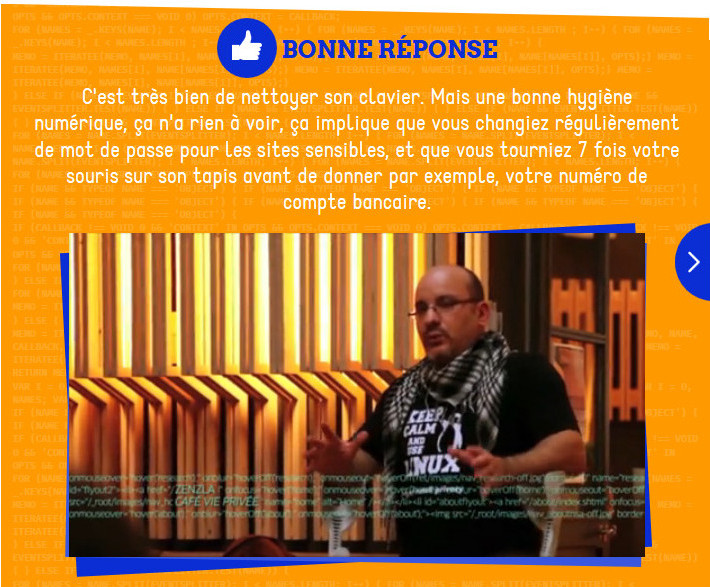
\includegraphics[scale=0.5] {./images/Quizz_HygieneNumerique_France4_7.jpg}
\end{center}
\end{frame}

%-----------------------------------------------
\begin{frame}
\begin{center}
\Huge{Donner des cours d'hygiène numérique}
\\~\\
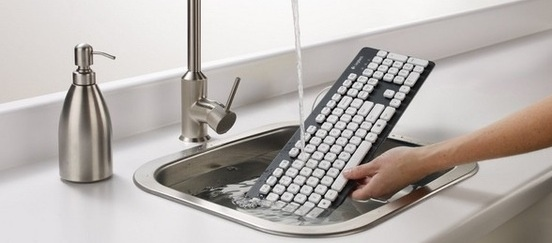
\includegraphics[scale=0.5]{./images/nettoyer_son_clavier.jpg}
\end{center}
\end{frame}

%----------------------------------------------------------------------------------------
\begin{frame}
\frametitle{L'hygiène numérique?}
\begin{block}{Une définition?}
\justifying{
L'hygiène est un ensemble de mesures destinées à prévenir les infections et l'apparition de maladies infectieuses.
\\
L'hygiène numérique, ce sont des règles destinées à mieux utiliser son ordinateur, en sécurité, de façon simple.
}
\end{block}
\huge{On va éviter la gastro informatique}

\end{frame}

%----------------------------------------------------------------------------------------
\begin{frame}
\frametitle{Un exemple}
\begin{block}{On me vole mon PC}
\justifying{
\begin{itemize}
\item  Quelles sont les données que je perds? Amène la notion de \emph{sauvegarde}.
\item  Quelles sont les données que l'on trouve? Amène la notion de \emph{chiffrement, de coffre fort numérique}.
\end{itemize}
}
\end{block}
\begin{center}
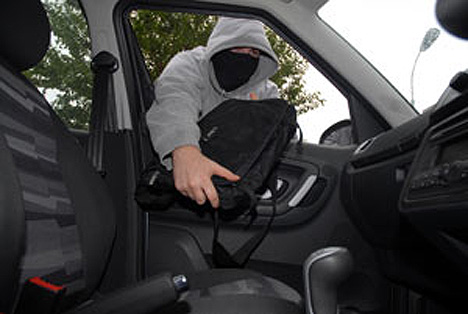
\includegraphics[scale=0.5] {./images/laptopthief.jpg}
\end{center}
\end{frame}

%----------------------------------------------------------------------------------------
\begin{frame}
\frametitle{D'autres exemples}
\begin{block}{Si je suis dans les temps :-)}
\justifying{
\begin{itemize}
\item \emph{Plus c'est long, plus c'est bon}
\item \emph{BelleMaman Genma utilise mon PC}
\item \emph{J'ai des hémoroïdes}
\item \emph{Donner ses clefs au comissariat}
\end{itemize}
}
\end{block}
\end{frame}

%-----------------------------------------------
\begin{frame}
\begin{center}
\Huge{Envie de vous lancer?}
\Huge{De vous impliquer à votre tour?}
\end{center}
\end{frame}


%-----------------------------------------------
\begin{frame}
\begin{center}
\Huge{Le Yakafokon}
\end{center}
\end{frame}


%-----------------------------------------------
\begin{frame}
\begin{center}
\Huge{Le monde associatif}
\end{center}
\end{frame}

%-----------------------------------------------
\begin{frame}
\frametitle{ALDILL}

\begin{block}{Association Lyonnaise pour le Développement de l'Informatique Libre}
\url{http://www.aldil.org/}
\end{block}
\begin{center}

\includegraphics[scale=0.5] {./images/Aldill.png}
\end{center} 
\end{frame}

%-----------------------------------------------
\begin{frame}
\frametitle{Sur Paris - Parinux}

\begin{block}{Premier Samedi du Libre (PSL)}
\justifying{Chaque premier samedi de chaque mois, les bénévoles des associations du Libre vous accueillent au Carrefour Numérique de la Cité des sciences et de l'industrie (CSI) pour une install party.\\ \url{http://premier-samedi.org/}
}
\end{block}
\begin{center}

\includegraphics[scale=0.5] {./images/parinux.png}
\end{center} 
\end{frame}
%-----------------------------------------------
\begin{frame}
\frametitle{Ubuntu Party}
\begin{block}{Ubuntu-fr}
Ubuntu Party : prochaine les 28 et 29 mai sur Paris.\\
\url{http://www.ubuntu-paris.org/}
\end{block}
\begin{center}
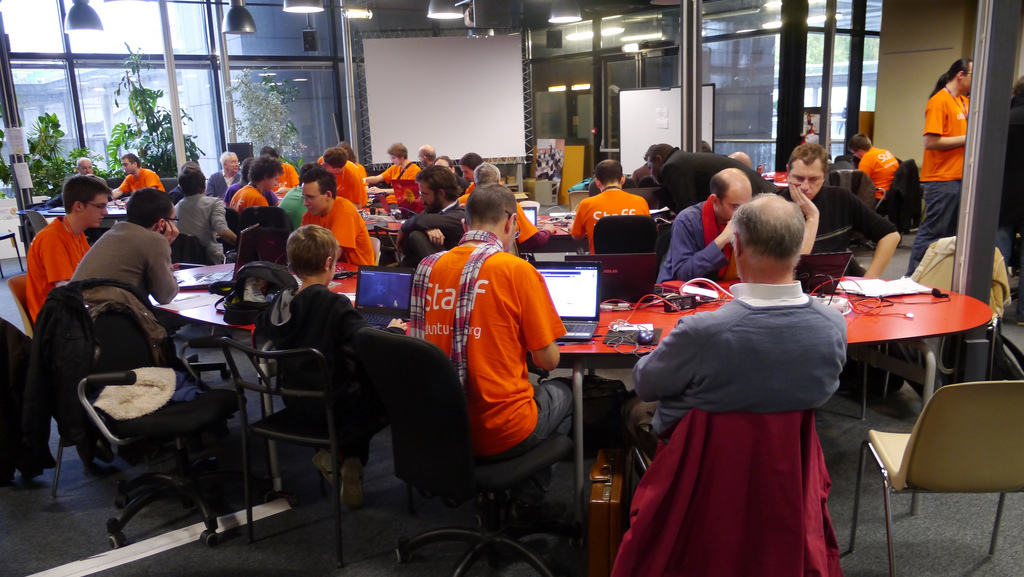
\includegraphics[scale=0.3] {./images/ubuntu-paris.jpg}
\end{center} 
\end{frame}
%-----------------------------------------------
\begin{frame}
\frametitle{Agenda du libre }
\begin{center}
\url{http://www.agendadulibre.org/}
\\
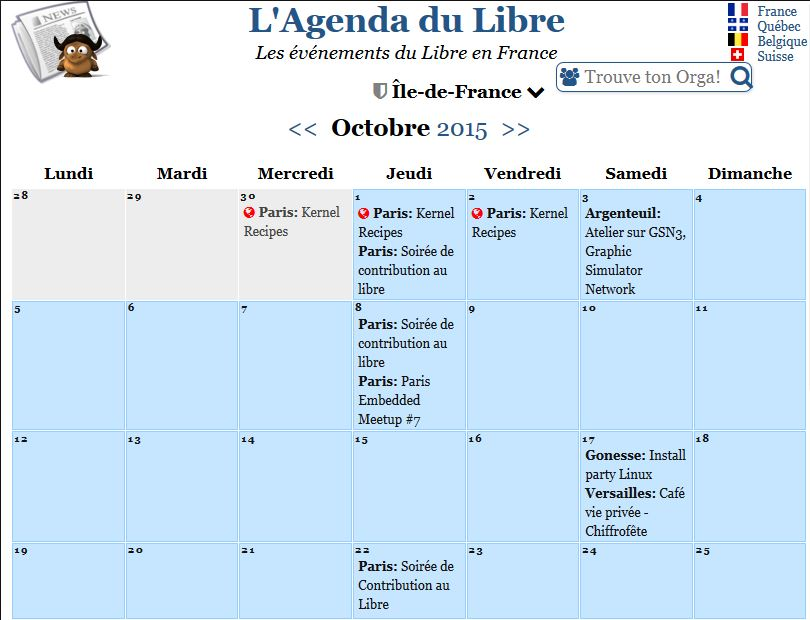
\includegraphics[scale=0.55] {./images/agenda-du-libre.jpg}
\end{center} 
\end{frame}

%----------------------------------------------------------------------------------------
\begin{frame}
\begin{center}
\Huge{Café vie privée, chiffrofête, cryptoparty}
\\~\\

\includegraphics[scale=0.3] {./images/LogoCafeViePrivee.jpg}
\end{center}
\end{frame}

%========================================================================================
\begin{frame}
\begin{center}
\Huge{Merci de votre attention}
\\
\Huge{Place aux questions.}
\\~\\

\includegraphics[scale=0.2] {./images/chat.jpg}
\end{center}
\end{frame}

%----------------------------------------------------------------------------------------
\begin{frame}
\frametitle{
\includegraphics[scale=0.4]{./images/Genma.jpg} \ \ \  Me contacter?}
\Huge{\centerline{Le Blog de Genma}}
\Huge{\centerline{http://genma.free.fr}}
\Huge{\centerline{~}}
\Huge{\centerline{Twitter : @genma}}
\end{frame}

%============================================================================================
\begin{frame}
\Huge{\centerline{ANNEXES}}
\end{frame}

%----------------------------------------------------------------------------------------
\begin{frame}
\frametitle{Aux détracteurs, trolls, critiques malvenues et aggressives...}
\begin{center}
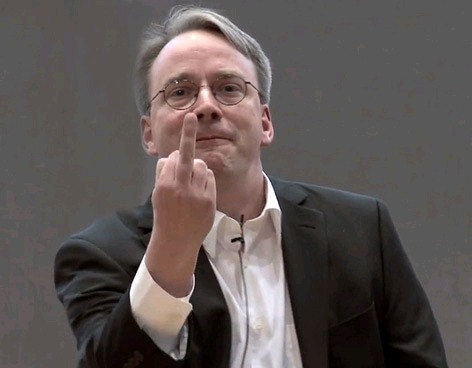
\includegraphics[scale=0.5] {./images/linus.jpg}
\end{center}
\end{frame}

%--------------------------------------------------------------------------------
\begin{frame}
\frametitle{Autonomie des individus parJérémie ZImmerman }
\begin{block}{Citation d'une interview donnée au podcast le Comptoir Sécu à l'occasion du FIC2016}
\justifying{
"On en a toujours parler les mains sur le clavier, les yeux sur l'écran.
Il faut parler de tout ça en des termes simples et en des termes politiques, éthiques.
Ce n'est pas y en a qu'est simple (Gmail, Mac etc.) et l'autre qui est compliqué. Non.
\\~\\Y en a qui est libre et l'autre qui est une prison.
Y en a un qui permet de comprendre, l'autre maintient dans l'ignorance
Y en a un qui permet de détenir collectivement le contrôle sur la machine, et l'autre dans lequel la machine te contrôle.
\\~\\C'est en ces termes là à mon avis qu'il faut expliquer ces choses là.
}\end{block}
\url{http://www.comptoirsecu.fr/2016/02/fic2016-2-jeremie-zimmermann-nicolas-diaz/}
\end{frame}

%----------------------------------------------------------------------------------------
\begin{frame}
\justifying{
Cette partie est une adaptation /s'inspire du retour d'expérience "Conseils à un libriste pour faire passer au libre" de Dada, qui est un texte mis à disposition selon les termes de la Licence Creative Commons Attribution - Partage dans les Mêmes Conditions 4.0 International. \url{http://www.dadall.info/blog}
}
\end{frame}

%------------------------------------------------
\begin{frame}
\begin{block}{Commencer simplement, par des logiciels courants}
\justifying{
\begin{itemize}
\item Firefox, Thunderbird et VLC sont les meilleurs moyens au monde pour faire glisser quelqu'un vers les logiciels libres.
\item  Ils regroupent les besoins de 90 \% des utilisateurs.
\end{itemize}
}
\end{block}

\begin{block}{Ne parlez pas de logiciel libre tout de suite}
\justifying{
\begin{itemize}
\item L'ordinateur est une boite noire. 
\item Personne n'y comprend rien et personne ne veut comprendre. 
\item Alors laissez tomber l'approche éthique de votre démarche si vous savez que la personne en face n'est pas sensible à ça. 
\end{itemize}
}
\end{block}
\end{frame}

\begin{frame}
\begin{block}{GNU/Linux, privateur, RMS...}
\justifying{
\begin{itemize}
\item Ne commencez à dire que Linux, c'est bien mieux que Windows.
\item Ne parlez pas de la philosophie, des 4 libertés, de RMS...
\item Parlez d'Ubuntu, dont le nom peut être connu.
\item ET NE PARLEZ PAS DE GNU/Linux.
\end{itemize}
}
\end{block}

\begin{block}{Ne commencez jamais par le système d'exploitation}
\justifying{
\begin{itemize}
\item Non parlez pas du fonctionnement du système d'exploitation. 
\item ne parlez pas de la ligne de commande qui est trop bien.
\end{itemize}
}
\end{block}
\end{frame}
%------------------------------------------------
\begin{frame}
\begin{block}{Refusez d'aider un utilisateur de logiciels piratés}
\justifying{
\begin{itemize}
\item Installer lui du logiciel libre.
 \item Non Gimp ce n'est pas Photoshop, il faut REAPPRENDRE, se créer de nouvelles habitudes.
\end{itemize}
}
\end{block}
\begin{block}{Assumez le Service Après Vente}
\justifying{
\begin{itemize}
\item Assumez le SAV. 
\item N'oubliez pas de configurer les mis à jour des versions d'Ubuntu vers les LTS suivantes uniquement.
\end{itemize}
}
\end{block}
\end{frame}

%------------------------------------------------
\begin{frame}
\begin{block}{Ne pas forcer le passage}
\justifying{
\begin{itemize}
\item Il ne sert à rien de se lever un jour en disant qu'untel va avoir le droit à son passage au libre. 
\item Il s'en fout, n'a pas connaissance des courants privateur et libre des logiciels. 
\item L'utilisateur d'un ordinateur veut que ça marche et n'aime pas le changement.
\end{itemize}
}
\end{block}

\begin{block}{Attendez que l'ordinateur se dégrade avant d'agir.}
\justifying{
\begin{itemize}
\item Prendre l'ordinateur d'un ami et lui installer quelque chose qu'il ne connait pas parce que vous vous trouvez ça bien, c'est trop souvent foncer dans le mur. 
\item Quand ça marche, ça marche et il ne veut surtout pas que ça change. 
\item Attendez qu'il veuille changer, qu'on lui répare l'ordinateur...
\end{itemize}
}
\end{block}
\end{frame}
\end{document}